\usetikzlibrary{positioning}
\chapter{Preliminares}\label{chapter:preliminares}

El objetivo de este trabajo es encontrar un sistema de ecuaciones diferenciales ordinarias (EDOs) compartimentales que describa un conjunto 
de puntos observados. Se asume que la din\'amica poblacional inicialmente no se conoce y que puede representarse mediante un grafo dirigido que 
define las posibles interacciones entre compartimentos; identificar dicha estructura es parte del proceso de modelado. 
Para ello, se propone un enfoque basado en algoritmos genéticos que explorara diferentes grafos dirigidos, donde cada nodo representa un compartimento 
y cada arco el flujo entre los nodos. A partir de cada grafo generado se construye un sistema de ecuaciones diferenciales compartimentales, que 
se evalúa mediante una función de costo, conocida como \textit{fitness}, que cuantifica su capacidad para ajustarse a los datos proporcionados.

En este capítulo se presentan los fundamentos teóricos necesarios para el desarrollo del trabajo: los sistemas de ecuaciones diferenciales ordinarias, 
los modelos compartimentales, el ajuste por mínimos cuadrados, el algoritmo genético con énfasis en sus operadores de selección, cruzamiento y mutación, 
y los métodos numéricos utilizados para la resolución de los sistemas propuestos, en particular Runge-Kutta y las fórmulas de diferenciación inversa. 
El capítulo está dividido en 5 secciones.

En la sección~\ref{sec:edos} se introducen los sistemas de ecuaciones diferenciales ordinarias, los cuales permiten describir matemáticamente los sistemas dinámicos 
generados a partir de los grafos. A continuación, la sección~\ref{sec:compartimental} aborda los sistemas compartimentales, que representan de forma estructurada el 
flujo de cantidades entre estados discretos o compartimentos. En la sección~\ref{sec:mincuad} se presenta el ajuste por mínimos cuadrados, para estimar los parámetros 
de los modelos a partir de datos observados. La sección~\ref{sec:metodos-numericos} se presentan los métodos numéricos que se emplean para resolver los sistemas de 
ecuaciones diferenciales asociados a los grafos evaluados, permitiendo obtener las trayectorias del sistema para su comparación con los datos reales. Finalmente, en 
la sección~\ref{sec:ag} está dedicada al algoritmo genético, describiendo sus operadores principales: selección, cruzamiento y mutación. Estos componentes conforman 
el mecanismo de búsqueda que permite explorar el espacio de posibles grafos que generan sistemas adecuados. 

\section{Sistemas de Ecuaciones Diferenciales Ordinarias}
\label{sec:edos}

Un sistema de ecuaciones diferenciales ordinarias es un conjunto de una o más ecuaciones que relacionan una función desconocida o un conjunto de funciones 
con respecto a una única variable independiente, a través de sus derivadas \cite{BoyceDiPrima17, Zill13}. Este tipo de sistemas describe cómo cambia una o varias 
cantidades en el tiempo, según una dinámica especificada por funciones conocidas.

Matemáticamente, un sistema de \( n \) EDOs de primer orden puede escribirse como:
\begin{align*}
\frac{dx_1}{dt} &= f_1(t, x_1, x_2, \ldots, x_n) \\
\frac{dx_2}{dt} &= f_2(t, x_1, x_2, \ldots, x_n) \\
&\vdots \\
\frac{dx_n}{dt} &= f_n(t, x_1, x_2, \ldots, x_n)
\end{align*}
donde \( x_1(t), x_2(t), \ldots, x_n(t) \) son funciones desconocidas que dependen de la variable independiente \( t \), y \( f_1, f_2, \ldots, f_n \) son funciones 
conocidas que describen las tasas de cambio de cada variable. Para obtener una solución específica del sistema, es necesario fijar condiciones iniciales del 
tipo \( x_i(t_0) = x_{i,0} \), que determinan el estado del sistema en un instante inicial \( t_0 \).

Los sistemas de EDOs son utilizados para modelar fenómenos dinámicos en biología \cite{murray2002}, física \cite{strogatz2015}, economía \cite{chiang2005} o 
ingeniería \cite{ljung1999}, donde las tasas de cambio de ciertas cantidades dependen del estado actual de esas y otras cantidades relacionadas \cite{Arnold73}. 
Existe una clase particular de sistemas de ecuaciones diferenciales ordinarias, conocidos como modelos compartimentales, a la que se dedica la siguiente sección, 
junto con su representación mediante grafos dirigidos.

\section{Sistemas de Ecuaciones Diferenciales Ordinarias Compartimentales}
\label{sec:compartimental}

Los sistemas de EDOs compartimentales son una herramienta matemática utilizada para describir la evolución de una cantidad que se distribuye entre distintos estados o 
compartimentos. Cada compartimento representa una parte diferenciada del sistema que se desea modelar, como puede ser un grupo de individuos en una población, 
una fase en un proceso químico o un estado de salud en una enfermedad \cite{murray2002,atkins2014}. Entre estos compartimentos existe un flujo que indica cómo la 
cantidad se transfiere de uno a otro.

Este tipo de modelos se emplea en ecología para representar la interacción entre especies \cite{Jacquez96}, en ingeniería química para modelar procesos de transporte 
de sustancias \cite{Godfrey83}, y en epidemiología para estudiar la propagación de enfermedades \cite{AndersonMay91}. En este último caso, uno de los modelos más 
conocidos es el modelo SIR, que clasifica a la población en tres compartimentos: susceptibles, infectados y recuperados. Las ecuaciones que describen su dinámica son:

\begin{align}
\frac{dS}{dt} &= -\beta SI, \\
\frac{dI}{dt} &= \beta SI - \gamma I, \\
\frac{dR}{dt} &= \gamma I,
\end{align}

donde:
\begin{itemize}
    \item \(S\) es la población susceptible,
    \item \(I\) es la población infectada,
    \item \(R\) es la población recuperada,
    \item \(\beta\) es la tasa de transmisión,
    \item \(\gamma\) es la tasa de recuperación.
\end{itemize}

Una forma natural de representar los compartimentos de un sistema y los flujos entre ellos es mediante grafos dirigidos, en los cuales los nodos corresponden a los 
compartimentos y las aristas representan las transferencias o interacciones entre ellos \cite{heesterbeek2012construction}. La Figura~\ref{fig:grafo-sir} muestra
un ejemplo del modelo SIR representado mediante un grafo.

A partir del grafo definido, se construye un sistema de ecuaciones diferenciales ordinarias que describe la evolución temporal de cada compartimento. La presencia de 
una arista dirigida desde el nodo \(X\) hacia el nodo \(Y\) indica que existe un flujo desde \(X\) hacia \(Y\); este flujo debe modelarse como una pérdida en la 
ecuación de \(X\), término negativo, y una ganancia en la de \(Y\), término positivo. La ausencia de una conexión entre dos compartimentos implica que no existe 
interacción directa entre ellos, lo cual se refleja en las ecuaciones como la falta de términos que involucren simultáneamente a ambas variables.

\begin{figure}[htbp]
    \centering
    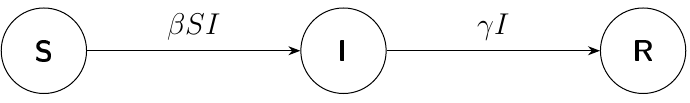
\includegraphics[width=0.7\textwidth]{Graphics/sir_graph.png}
    \caption{Grafo del modelo compartimental SIR.}
    \label{fig:grafo-sir}
\end{figure}

Es fundamental que la modelación de estos flujos preserve coherencia en la representación matemática: cada transferencia entre compartimentos debe estar reflejada 
simétricamente como salida en una ecuación y entrada en otra. Si un flujo aparece restando en una ecuación pero no sumando en otra, se estaría introduciendo una 
pérdida neta de cantidad sin justificación física o biológica, lo cual constituye un error en la formulación del modelo compartimental. Esta correspondencia entre el 
grafo y el sistema de ecuaciones asegura, por ejemplo, la conservación de la cantidad total cuando el sistema así lo requiere, y ofrece además una interpretación 
estructural clara del proceso dinámico.

Cabe mencionar que también pueden existir flujos externos que no provienen de otro compartimento, como nacimientos en una población o entradas de materia desde una 
fuente externa. En estos casos, el término correspondiente se incorpora directamente en la ecuación del nodo de destino, sin necesidad de que exista otro nodo de 
origen en el grafo.

Identificar la estructura del grafo compartimental es un paso fundamental en el proceso de modelado, ya que determina qué interacciones se consideran posibles dentro 
del sistema de EDOs compartimentales. Sin embargo, conocer dicha estructura no es suficiente. Las ecuaciones diferenciales asociadas incluyen parámetros que determinan 
la intensidad o velocidad de cada flujo, y estos parámetros, en general, no se conocen con antelación. Por ello, deben estimarse a partir de datos observados. Una de 
las técnicas para este propósito es el ajuste por mínimos cuadrados, que será presentado en la sección siguiente.

\section{Ajuste por Mínimos Cuadrados}
\label{sec:mincuad}

El método de mínimos cuadrados es una técnica matemática ampliamente utilizada para ajustar modelos a datos observados, cuyo objetivo es encontrar los 
parámetros de un modelo que mejor expliquen los datos disponibles. Este método consiste en minimizar la suma de los cuadrados de las diferencias entre 
los valores observados y los valores estimados por el modelo \cite{Stigler81}.

Dado un conjunto de \( m \) observaciones \(\{t_k, y_k\} \in \mathbb{R} \times \mathbb{R}^m\), una función modelo \( f(t, \mathbf{p}) \) dependiente de un vector de 
parámetros \( \mathbf{p} \in \mathbb{R}^k \), y una función de error definida por la diferencia entre el valor observado \( y_k \) y el valor predicho por el modelo 
\( f(t_k, \mathbf{p}) \), se define la función objetivo:

\[
SSR(\mathbf{p}) = \sum_{k=1}^{m} [y_k - f(t_k, \mathbf{p})]^2,
\]

donde \( SSR \) (por sus siglas en inglés, \textit{Sum of Squared Residuals}) representa la suma de los cuadrados de los residuos. El problema consiste en encontrar 
el vector de parámetros \( \mathbf{p}^* \) que minimiza esta suma, es decir:

\[
\mathbf{p}^* = \arg \min_{\mathbf{p}} SSR(\mathbf{p}).
\]

Este enfoque permite ajustar modelos paramétricos cuando se conoce la forma funcional general de la relación entre las variables. Al minimizar el error 
cuadrático medio, se obtiene una estimación de los parámetros que proporciona la mejor aproximación posible al conjunto de datos, bajo el supuesto de 
errores distribuidos normalmente.

En el contexto de este trabajo, el método de mínimos cuadrados se utilizará para estimar los valores de los parámetros presentes en las ecuaciones diferenciales 
de los sistemas compartimentales generados a partir de grafos. A partir de un conjunto de datos observados, se buscará minimizar la diferencia entre las 
soluciones del modelo y los datos, de modo que los parámetros ajustados representen de forma adecuada la dinámica observada.

En este caso, el modelo ya no está definido por una expresión explícita como \( f(t, \mathbf{p}) \), sino por un sistema de ecuaciones diferenciales cuya solución 
depende de los parámetros. Esto implica que, para cada evaluación del error en el proceso de optimización, es necesario resolver el sistema de EDOs asociado. 
Por tanto, la integración numérica se convierte en un componente central del procedimiento. A continuación se introduce los m\'etodos num\'ericos, que serán utilizados 
para calcular las soluciones aproximadas de estos sistemas diferenciales.

\section{M\'etodos Num\'ericos}
\label{sec:metodos-numericos}

Los sistemas de EDOs aparecen con frecuencia en la modelación de fenómenos dinámicos en diversas disciplinas científicas \cite{Boyce2012}. En la mayoría de los casos, 
estos sistemas no admiten soluciones analíticas, por lo que es necesario recurrir a métodos numéricos para obtener aproximaciones de su comportamiento a lo largo 
del tiempo \cite{Burden2011}.

Esta sección presenta dos enfoques clásicos de integración numérica que permiten resolver EDOs de forma eficiente y precisa, según las características del problema. 
En primer lugar, se introduce el método de Runge-Kutta \cite{Burden2011}, ampliamente utilizado por su simplicidad y buen desempeño en una amplia gama de aplicaciones. 
Posteriormente, se describen las Fórmulas de Diferenciación Inversa (BDF), que ofrecen una alternativa robusta para sistemas que presentan rigidez \cite{Hairer1996}. 
A continuación, se detalla el método de Runge-Kutta y sus principales propiedades.

\subsection{Runge-Kutta}

Los métodos de Runge-Kutta constituyen una familia de algoritmos numéricos diseñados para obtener soluciones aproximadas de ecuaciones diferenciales ordinarias. 
Estos métodos se basan en cálculos iterativos que permiten avanzar paso a paso en la solución del sistema. Dentro de esta familia, el método de Runge-Kutta de orden 
4 es ampliamente utilizado por su equilibrio entre precisión y eficiencia computacional \cite{Fehlberg70, DormandPrince80}.

El método Runge-Kutta con control del tamaño de paso se basa en la combinación de dos fórmulas de diferentes órdenes: una de cuarto y otra de quinto. Ambas se utilizan 
de forma simultánea en cada paso de integración. La estimación del error local de truncamiento se obtiene como la diferencia entre estas dos soluciones. Esta 
característica permite que el método implemente un mecanismo de control de paso adaptativo: si el error estimado supera una tolerancia establecida, el tamaño del paso 
se reduce; si el error es pequeño, el paso se incrementa. Este ajuste dinámico del paso hace que el método sea especialmente eficiente en regiones donde la solución 
varía lentamente, y preciso en zonas de alta variación \cite{HairerNorsettWanner93}.

Para una EDO de la forma:

\[
\frac{dy}{dt} = f(t, y), \quad y(t_0) = y_0,
\]

el método de Runge-Kutta de orden 4 clásico calcula una aproximación \( y_{n+1} \) mediante la siguiente fórmula:

\[
\begin{aligned}
k_1 &= f(t_n, y_n), \\
k_2 &= f\left(t_n + \frac{h}{2}, y_n + \frac{h}{2}k_1\right), \\
k_3 &= f\left(t_n + \frac{h}{2}, y_n + \frac{h}{2}k_2\right), \\
k_4 &= f(t_n + h, y_n + hk_3), \\
y_{n+1} &= y_n + \frac{h}{6}(k_1 + 2k_2 + 2k_3 + k_4),
\end{aligned}
\]

donde \( h \) es el tamaño del paso y los \( k_i \) son pendientes intermedias que evalúan la función \( f \) en distintos puntos del intervalo. Esta fórmula 
proporciona una estimación de cuarto orden, lo que significa que el error local de truncamiento es proporcional a \( h^5 \).

El método Runge-Kutta agrega una segunda estimación de quinto orden que permite estimar el error cometido en el paso. A partir de esa estimación, se decide si aceptar 
el paso, si el error es pequeño, o repetirlo con un valor de \( h \) reducido, si el error es grande. Esta propiedad lo hace particularmente útil cuando se trabaja 
con soluciones que tienen regiones con cambios rápidos y otras más suaves\cite{HairerNorsettWanner93}.

En este trabajo, el método Runge-Kutta se utilizará para resolver numéricamente los sistemas de ecuaciones diferenciales compartimentales generados a partir de grafos, 
especialmente en aquellos casos en los que el sistema no presenta rigidez y puede ser tratado eficientemente mediante un esquema explícito. Sin embargo, cuando los 
modelos compartimentales introducen escalas de tiempo muy distintas o propiedades que hacen al sistema rígido, será necesario recurrir a métodos más adecuados para 
tales situaciones. En la siguiente sección se presentarán las Fórmulas de Diferenciación Inversa, una alternativa robusta y estable para abordar este tipo 
de problemas.

\subsection{Fórmulas de Diferenciación Inversa}

Las Fórmulas de Diferenciación Inversa (\textit{Backward Differentiation Formulas}, BDF) son una familia de métodos implícitos multipaso para la integración numérica de 
EDOs, particularmente efectivos para resolver sistemas rígidos \cite{Gear71, HairerWanner96}. Una BDF de orden $s$ aproxima la 
derivada $y'(t_{n+1})$ utilizando los valores de la solución en $s+1$ puntos temporales anteriores y actuales: $t_{n+1}, t_n, \ldots, t_{n+1-s}$. La fórmula 
general es:
\[
\sum_{k=0}^{s} \alpha_k y_{n+1-k} = h \beta_0 f(t_{n+1}, y_{n+1}),
\]
donde $h$ es el tamaño del paso, y $\alpha_k, \beta_0$ son coeficientes que dependen del orden $s$. Al ser métodos implícitos (ya que $y_{n+1}$ aparece en ambos 
lados de la ecuación, a través de $f(t_{n+1}, y_{n+1})$), requieren resolver una ecuación en cada paso de tiempo, a menudo mediante métodos 
iterativos como Newton-Raphson\cite{BurdenFaires2011}.

La principal ventaja de los métodos BDF es su excelente estabilidad al resolver sistemas rígidos. Un sistema rígido es aquel que involucra escalas de tiempo muy 
diferentes, donde algunos componentes de la solución cambian muy rápidamente mientras otros lo hacen lentamente. En estos casos, los métodos explícitos como 
Runge-Kutta pueden requerir tamaños de paso extremadamente pequeños para evitar errores numéricos o inestabilidades. En cambio, los métodos BDF permiten utilizar 
pasos de integración mucho más grandes sin comprometer la precisión ni la estabilidad de la solución, lo que los convierte en una opción más eficiente para este 
tipo de problemas \cite{AscherPetzold98}.

Hasta este punto, se ha planteado el problema de estimar los parámetros de un modelo definido por un sistema de ecuaciones diferenciales, para lo cual es necesario 
resolver dichas ecuaciones en cada paso del proceso de ajuste. Esto justifica la introducción de los métodos de integración numérica, como Runge-Kutta y BDF, que 
permiten obtener soluciones aproximadas del sistema en función de los parámetros. Sin embargo, aún no se ha definido cómo construir el sistema dinámico en cuestión. 
Dado que la estructura del modelo compartimental no se conoce de antemano, es necesario generar distintas configuraciones posibles del sistema, lo cual equivale 
a explorar el espacio de grafos dirigidos que determinan qué compartimentos interactúan entre sí. Esta tarea, al implicar una búsqueda combinatoria compleja en el 
espacio de posibles grafos dirigidos, será abordada mediante el uso de algoritmos genéticos, que se introducen en la próxima sección como herramienta principal para 
la exploración estructural del sistema.

\section{Algoritmo Genético (AG)}
\label{sec:ag}

El Algoritmo Genético es una metaheurística de optimización y búsqueda inspirada en el proceso de selección natural y los principios de la genética biológica. 
Fue propuesto inicialmente por Holland \cite{Holland75} y posteriormente desarrollado y aplicado en una amplia variedad de contextos por diversos autores, 
entre ellos Goldberg \cite{Goldberg89}. Forma parte de la familia de los algoritmos evolutivos, los cuales han sido formalizados y sistematizados en obras como 
la de Eiben y Smith \cite{EibenSmith15}.

Los algoritmos genéticos se basan en la conservación y modificación de una población de soluciones candidatas, también llamadas individuos o cromosomas.

Cada individuo representa una posible solución al problema que se desea resolver, codificada en una estructura manipulable, como una cadena de bits, una lista de 
enteros, un grafo dirigido, entre otros. A cada solución se le asigna un valor de aptitud, conocido como \textit{fitness}, el cual cuantifica qué tan buena es con 
respecto a la función objetivo.

La población se modifica a lo largo de sucesivas generaciones mediante la aplicación iterada de operadores genéticos como la selección, el cruzamiento y la mutación. 
A través de estos mecanismos, se combinan y modifican estructuras existentes para explorar el espacio de búsqueda, con el objetivo de encontrar 
soluciones cada vez mejores.

En este trabajo, el algoritmo genético se utilizará para explorar el conjunto de posibles grafos dirigidos que definen modelos compartimentales. Cada individuo 
en la población representará un grafo, donde los nodos corresponden a compartimentos y los arcos representan flujos entre ellos. A partir de cada grafo, se construye 
un sistema de EDOs compartimentales que modela la dinámica del sistema. El desempeño de cada modelo se evalúa resolviendo este sistema y comparando la solución 
obtenida con los datos observados, mediante una función de aptitud. Esta función combina el error cuadrático medio entre las trayectorias simuladas y los datos 
originales, junto con penalizaciones por características estructurales no deseadas. Estas penalizaciones incluyen, por ejemplo, la no conservación de la población total 
y una complejidad excesiva del grafo, medida según la cantidad de aristas. Esta función compuesta permite favorecer modelos que no solo se ajusten bien a los datos, 
sino que también respeten principios estructurales deseables como simplicidad y coherencia dinámica.

En las siguientes secciones se describen con detalle los componentes fundamentales del algoritmo genético 
aplicado: los operadores de cruzamiento, mutación y selección, responsables de la evolución de la población de grafos a lo largo del proceso de optimización.

\subsection{Cruzamiento}

La función del operador de cruzamiento, también conocido como recombinación, es combinar la información de dos o más individuos seleccionados denominados padres, 
para generar nuevos individuos denominados hijos, que hereden características de ambos progenitores. Este proceso está inspirado en la reproducción sexual y tiene 
como objetivo explorar nuevas regiones del espacio de búsqueda, favoreciendo la diversidad genética dentro de la población \cite{Holland75}.

En contextos tradicionales donde los individuos se representan mediante vectores numéricos, existen operadores de cruzamiento bien conocidos como el 
cruzamiento aritmético o el \textit{Simulated Binary Crossover}, comúnmente utilizado en optimización continua \cite{DebAgrawal95}. Sin embargo, cuando los individuos 
representan estructuras más complejas como grafos dirigidos, es necesario adaptar el operador de cruzamiento a esta representación.

En este trabajo, cada individuo representa un grafo dirigido con una cantidad fija de nodos, correspondiente al número de variables observadas en los datos. El 
cruzamiento entre dos grafos consiste en generar un nuevo grafo que combine subestructuras de ambos padres. Existen diversas formas de implementar este operador 
sobre grafos; una de las más intuitivas es el cruzamiento por unión parcial, donde se toma un subconjunto de aristas del primer padre y otro subconjunto del segundo, 
y se combinan para formar un nuevo conjunto de aristas en el descendiente. 

La Figura~\ref{fig:cruzamiento-uparcial} muestra un ejemplo de cruzamiento por unión parcial.

\begin{figure}[htbp]
    \centering
    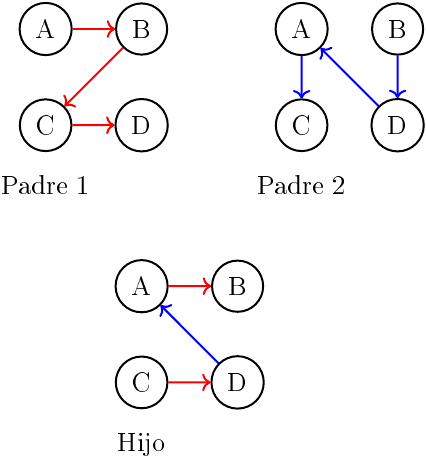
\includegraphics[width=0.35\textwidth]{Graphics/cruzamiento_pree_uparcial.png}
    \caption{Ejemplo de cruzamiento por unión parcial.}
    \label{fig:cruzamiento-uparcial}
\end{figure}

En el cruzamiento por intersección y expansión, se parte de las aristas comunes entre los dos padres y luego se añaden algunas aristas 
exclusivas de cada padre , seleccionadas aleatoriamente, manteniendo un equilibrio entre explotación y exploración. 

La Figura~\ref{fig:cruzamiento-intexp} muestra un ejemplo de cruzamiento por intersección y expansión.

\begin{figure}[htbp]
    \centering
    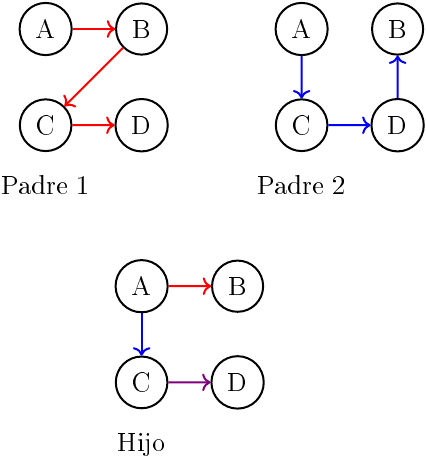
\includegraphics[width=0.35\textwidth]{Graphics/curzamiento_pree_intexp.png}
    \caption{Ejemplo de cruzamiento por intersección y expansión.}
    \label{fig:cruzamiento-intexp}
\end{figure}

La aplicación del cruzamiento en grafos permite generar nuevas topologías de modelos compartimentales, promoviendo la innovación estructural dentro del proceso 
evolutivo. Sin embargo, para evitar la convergencia prematura y fomentar la exploración del espacio de búsqueda, también es necesario introducir variaciones 
aleatorias en los hijos. Estas modificaciones puntuales se realizan a través del operador de mutación, el cual se describirá en la siguiente sección.


\subsection{Mutación}

El operador de mutación introduce variaciones aleatorias en los individuos de la población \cite{Goldberg89}. Su objetivo es mantener la diversidad dentro del 
algoritmo genético, evitando que la población converja prematuramente hacia soluciones subóptimas. A diferencia del cruzamiento, que combina información preexistente, 
la mutación genera nuevas características que no estaban presentes en los padres, permitiendo así una exploración más amplia del espacio de búsqueda.

En representaciones numéricas tradicionales, existen operadores como la mutación polinomial o la mutación gaussiana, que consisten en pequeñas perturbaciones sobre 
los valores de los genes \cite{DebBeyer01Final}. No obstante, cuando los individuos representan estructuras discretas como grafos, la mutación debe adaptarse a ese 
contexto.

La mutación aplicada a grafos consiste en modificar aleatoriamente su topología, afectando directamente los arcos que conectan los nodos. Algunas de las operaciones 
de mutación más comunes en este contexto incluyen:

\begin{itemize}
    \item \textbf{Adición de una arista:} se inserta un nuevo arco entre dos nodos que no estaban previamente conectados.
    \item \textbf{Eliminación de una arista:} se remueve un arco existente del grafo, simplificando su estructura.
    \item \textbf{Reversión de una arista:} se invierte la dirección de un arco existente, modificando el flujo entre compartimentos.
\end{itemize}

La Figura~\ref{fig:mutaciones-grafo-pree} muestra un ejemplo de cada una de las mutaciones mencionadas. 

\begin{figure}[htbp]
    \centering
    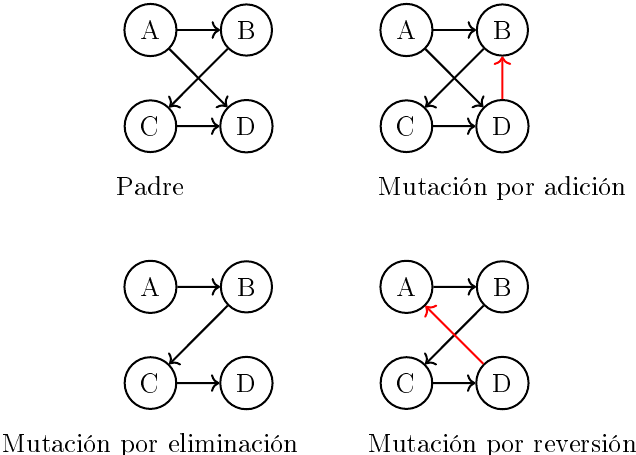
\includegraphics[width=0.5\textwidth]{Graphics/mutacion_pree.png}
    \caption{Ejemplo de mutaciones sobre grafo.}
    \label{fig:mutaciones-grafo-pree}
\end{figure}

Estas pequeñas modificaciones permiten que los hijos exploren regiones del espacio de grafos no alcanzables solo mediante cruzamiento, incrementando así la capacidad 
del algoritmo para descubrir modelos más adecuados. Las mutaciones se aplican típicamente con baja probabilidad, para evitar que la búsqueda se vuelva puramente 
aleatoria y pierda la dirección evolutiva basada en el desempeño.

Una vez generados y modificados los nuevos individuos, es necesario determinar cuáles serán preservados para la siguiente generación. Este proceso se lleva a cabo 
mediante el operador de selección, que se presentará en la próxima sección.


\subsection{Selección}

La selección es el proceso mediante el cual se eligen los individuos de la población actual que participarán en la generación de la siguiente. Este 
operador guía la presión evolutiva del algoritmo genético, favoreciendo la reproducción de aquellos individuos que presentan mayor desempeño según el \textit{fitness}. 
La probabilidad de ser seleccionado está relacionada directamente con la calidad de la solución, de modo que los modelos más prometedores tienen más oportunidades 
de transmitir sus estructuras a las generaciones futuras \cite{Goldberg89}.

Existen diversos métodos de selección, cada uno con características particulares. En la selección por ruleta, también llamada selección proporcional, 
la probabilidad de elegir un individuo es proporcional a su aptitud relativa dentro de la población. En la selección por torneo, se elige al azar un 
subconjunto pequeño de individuos y se selecciona el mejor entre ellos, un proceso que introduce competencia local. Finalmente, la selección por rango 
ordena a los individuos por aptitud y asigna probabilidades en función de su posición en el ranking, lo que suaviza las diferencias extremas y mantiene diversidad \cite{BlickleThiele96}.

Cuando los individuos representan grafos dirigidos, como en este trabajo, la función de aptitud depende no solo del ajuste del modelo a los datos 
medido mediante el error cuadrático medio, sino también de propiedades estructurales del grafo como su complejidad y la conservación de la población total. 
Por tanto, la selección favorece grafos que generan modelos compartimentales tanto precisos como coherentes desde el punto de vista dinámico y estructural.

Con el operador de selección se completa el ciclo evolutivo del algoritmo genético, permitiendo avanzar hacia generaciones sucesivas con individuos que combinan 
estructuras y comportamientos dinámicos. De esta manera, el algoritmo explora el espacio de modelos compartimentales.

Hasta aquí se han presentado los conceptos fundamentales necesarios para el desarrollo de esta tesis, incluyendo los sistemas de ecuaciones diferenciales, 
modelos compartimentales, métodos numéricos para su resolución, y el uso de algoritmos genéticos.

En el siguiente capítulo se describirá paso a paso cómo se construyen los sistemas de ecuaciones
diferenciales ordinarias compartimentales a partir de los grafos, y cómo se calcula el valor del \textit{fitness} que guía la evolución de las soluciones hacia modelos dinámicos.
